\pagenumbering{roman}

\renewcommand*\figurename{Abbildung}
\renewcommand*\tablename{Tabelle}

\newpage

\renewcommand*\contentsname{Inhaltsverzeichnis}
{
\hypersetup{linkcolor=}
\setcounter{tocdepth}{3}
\tableofcontents
}
\setstretch{1.5}

\newpage

\hypertarget{lot}{%
\subsection{Tabellenverzeichnis}\label{lot}}

\begin{table}[!hbt]
\caption{Zusammenhang zwischen Feuchtigkeit und Stadtwachstum}
\label{tbl1}
\centering
\begin{threeparttable}
  \begin{tabular}{llll} 

    \toprule
                                                & (1)      & (2)       & (3)        \\ 
    \midrule
    $\Delta$ moisture                           & -0.0761  & -1.064*** & -1.164***  \\
                                                & (0.180)  & (0.360)   & (0.354)    \\
    $\Delta$ moisture×(9 – \#modern industries) & ~        & 0.116***  & ~          \\
                                                & ~        & (0.0414)  & ~          \\
    $\Delta$ moisture×(14 – \#all industries)   & ~        & ~         & 0.0824***  \\
                                                & ~        & ~         & (0.0263)   \\
    (9 – \#modern industries)/1000              & ~        & -0.51     & ~          \\
                                                & ~        & (1.22)    & ~          \\
    (14 – \#all industries)/1000                & ~        & ~         & 0.131      \\
                                                & ~        & ~         & (0.727)    \\
    Initial share urban/1000                    & -48.9*** & -55.0***  & -52.0***   \\
                                                & (5.53)   & (8.79)    & (8.15)     \\
    ln(distance to coast)/1000                  & 1.43     & 1.55      & 1.47       \\
                                                & (1.89)   & (1.87)    & (1.89)     \\
    \bottomrule
    \end{tabular}
    
    \begin{tablenotes}
       \item \small Notes: Each column is a separate regression with 717 observations for 359 districts. The   dependent variable is growth in the urbanization rate. 9 and 14 are the maximum number of modern and total industries, respectively, in any district. Robust standard errors, clustered by district, are in parentheses. All specifications include country year fixed effects. * p < 0.1, ** p < 0.05, *** p < 0.01 
    \end{tablenotes}


\end{threeparttable}
\end{table}

\hspace{0.1em}

\begin{table}[!hbt]
\caption{Zusammenhang zwischen Feuchtigkeit und Einkommen}
\label{tbl2}
\centering
\begin{threeparttable}
  \begin{tabular}{lllll} 
    \toprule
                                                    & (1)      & (2)       & (3)       & (4)         \\ 
    \midrule
    $\Delta$ ln(rain(t))                            & -0.0124  & -0.207*** & -0.170*** & -0.0798***  \\
                                                    & (0.0124) & (0.0691)  & (0.0549)  & (0.0153)    \\
    $\Delta$ ln(rain(t))×(10 – \#modern industries) & ~        & 0.0199*** & ~         & ~           \\
                                                    & ~        & (0.00720) & ~         & ~           \\
    $\Delta$ ln(rain(t))×(14 – \#all industries)    & ~        & ~         & 0.0116*** & ~           \\
                                                    & ~        & ~         & (0.00424) & ~           \\
    $\Delta$ ln(rain(t))×1(ag/GDPgt;30)             & ~        & ~         & ~         & 0.107***    \\
    ~                                               & ~        & ~         & ~         & (0.0223)    \\
    \bottomrule
  \end{tabular}
  
  \begin{tablenotes}
       \item \small Notes: Each column is a separate regression with 1158 cities (18,528 obs). The dependent variable is $\Delta$ln(lights adjusted digital number). 10 and 14 are the maximum number of modern and total industries, respectively, in any city. Robust standard errors, clustered by district, are in parentheses. All specifications include year fixed effects * p < 0.1, ** p < 0.05, *** p < 0.01 
    \end{tablenotes}

\end{threeparttable}
\end{table}

\hypertarget{lof}{%
\subsection{Abbildungsverzeichnis}\label{lof}}

\begin{figure}[H]

{\centering 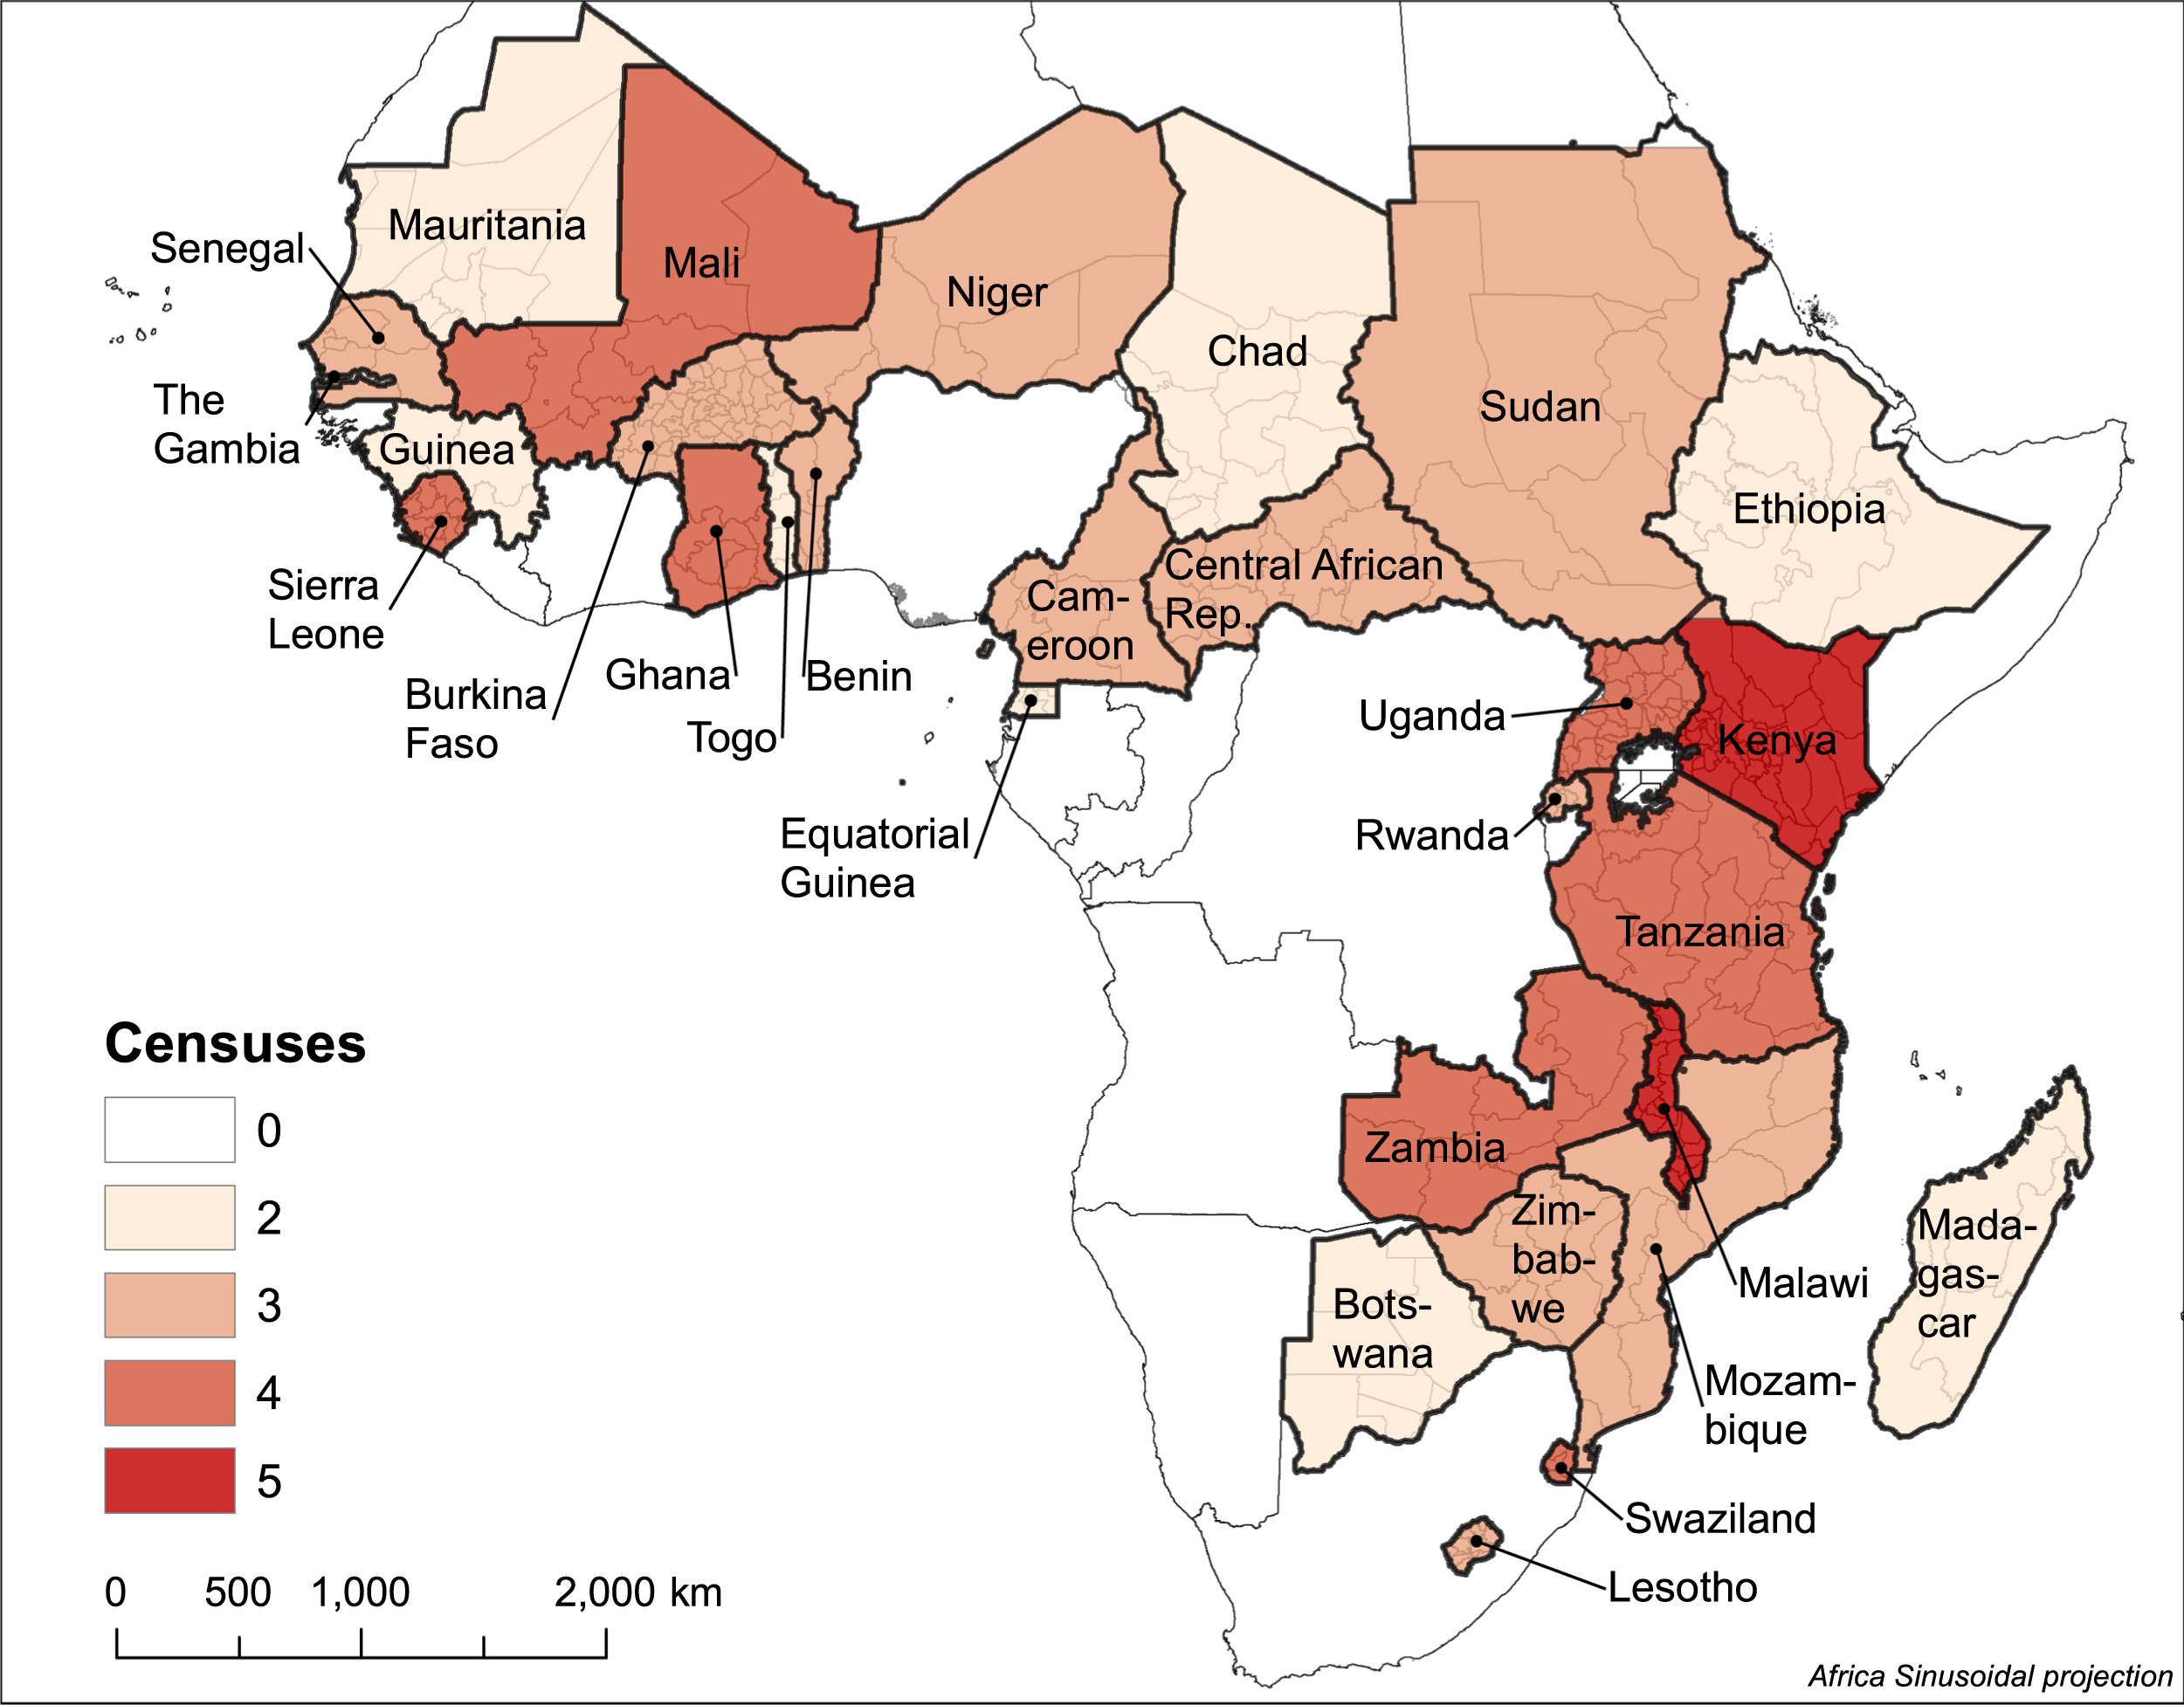
\includegraphics[width=0.7\textwidth]{../../images/2022-06-28_10-00-00.jpg}

}

\caption{Zensusdistrikte des Datensatzes}


{\centering 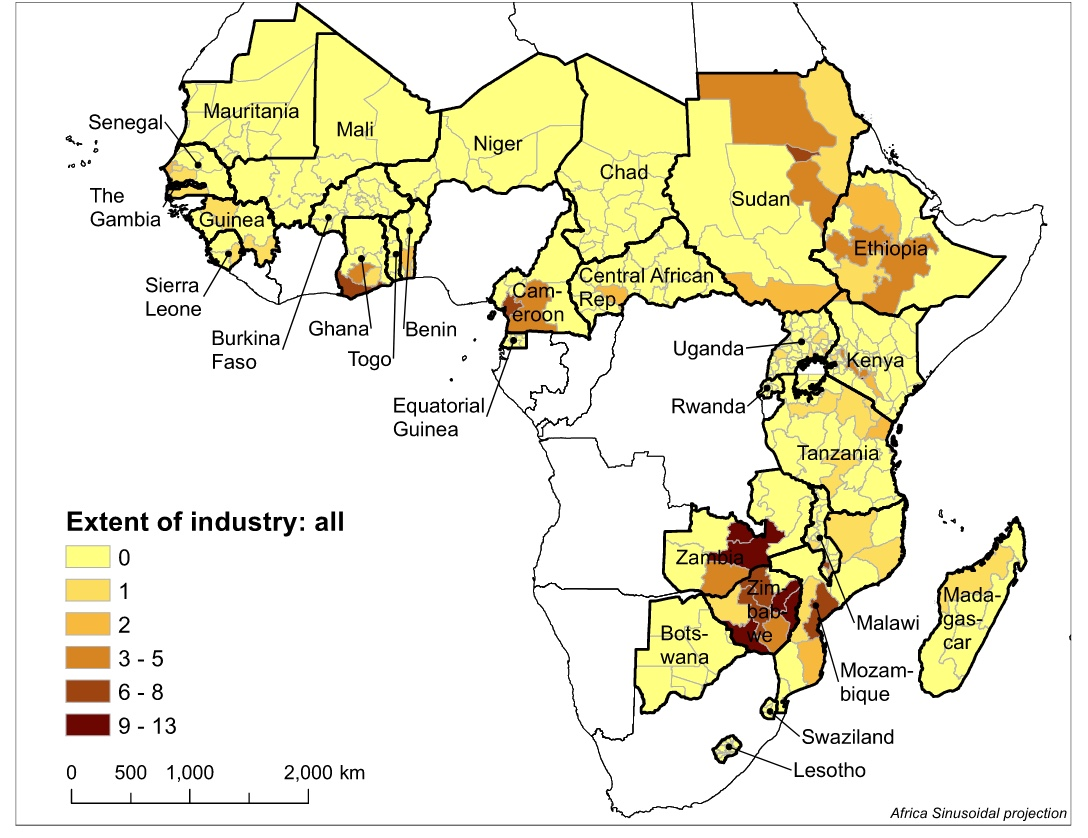
\includegraphics[width=0.7\textwidth]{../../images/2022-06-28_10-00-01.jpg}

}

\caption{Standorte der Industrien}

\end{figure}

\newpage
\pagenumbering{arabic}

